%Add [H] to tables and images.
\documentclass{maaprb}
%    If you need symbols beyond the basic set, uncomment this command.
\usepackage{amssymb}
\usepackage{float}
\usepackage{tcolorbox}
\usepackage{mdframed}
\usepackage{tikz}
\usepackage{graphicx}
\usepackage{float}
\usepackage{booktabs}
\usepackage{epigraph}
\usepackage{hyperref}
\usepackage{natbib}
\usepackage{forloop}
\usepackage{pgfmath}
\usepackage{etoolbox}
\usepackage{ifthen}
\usepackage{answers}
\usepackage{cancel}
\usepackage{draftwatermark}
% Watermark
\SetWatermarkLightness{ 0.9 }
\SetWatermarkText{DRAFT}
\SetWatermarkScale{ 3 }
%Expected Value
\newcommand{\E}[1]{\mathbb{E}({#1})}
%LCM command
\DeclareMathOperator*{\lcm}{lcm}
%true and false
\DeclareMathOperator*{\true}{true}
\DeclareMathOperator*{\false}{false}
% Points commad
\newcommand{\points}[1]{[$#1 \star$]}
% Setup counters
\newcounter{hindex}\setcounter{hindex}{0}
\newcounter{hintcounter}\setcounter{hintcounter}{0}
% Define \addhint and \gethint
\newcommand\addhint[1]{%
	\stepcounter{hintcounter}%
	\ref{hint:\thehintcounter}%
	\expandafter\gdef\csname hintlist\thehintcounter\endcsname{#1}%
}
\newcommand\gethint[1]{%
	\item \csname hintlist#1\endcsname \label{hint:#1}
}
\newenvironment{hint}{\footnotesize \normalfont \textbf{Hints}:}{\hspace{-0.5ex}}
\pgfmathsetseed{65536} % or any other number: sets the random seed

\newtheorem{theorem}{Theorem}[chapter]
\newtheorem{lemma}[theorem]{Lemma}

\theoremstyle{definition}
\newtheorem{definition}[theorem]{Definition}
\newtheorem{example}[theorem]{Example}
\newtheorem{xca}[theorem]{Exercise}

\theoremstyle{remark}
\newtheorem{remark}[theorem]{Remark}

\numberwithin{section}{chapter}
\numberwithin{equation}{chapter}
\setcounter{chapter}{-3}

\setcounter{chapter}{0}
\title{Doorway to Math Olympiads}
\author{Arjun Agarwal}
\begin{document}
\frontmatter
\maketitle
\mainmatter
\chapter{Permutations and Combinations and a pinch of Probability}
I'll begin this book with what we first learnt math as, counting.
\begin{example}
Cricket t-shirts have 2-digit numbers on them using six possible digits: $0, 1, 2, 3, 4, 5$ How many 
different t-shirts can be formed?
\end{example}
While we can write down all the possible t-shirt numbers and count them, we can do something 
faster and more beautiful. The first digit can be any of the $6$ given digits, and so can the
 second. As they are completely independent, we can simply multiply them.\par
So we have $6 \times 6=36$ such T-Shirts.
\begin{example}
How many $4$ digit numbers can be formed using the digits $1, 2, 3$ and $4$ (Without repetition).
\end{example}
This question is similar as while we can simply try to write all the numbers and then just count, 
but it is smarter to do something else.\par
This means we have $4$ choices for the thousands digit. As one number is now used, we only have
 $3$ choices for the hundreds digit. As two numbers are now used, we have only $2$ choices for 
 the tens digit. With all other numbers used, the last digit will be used as the one's digit, 
 leaving us with only $1$ choice. As all these choices are independent, we say that we can make 
 $4 \times 3 \times 2 \times 1 = 24$\par
Let's explore this new type of counting a bit more.
\section{Fundamental Principle of Counting}
\begin{example}
A person can travel from city $A$ to city $B$ via Road (Car/Bus/Bike), Train 
(Express/Mail) or Flight (Economy/Business). In how many ways can a person go from city A to city B?
\end{example}
Pretty standard, right? We can simply count the ways as $\text{Number of Road ways}
+\text{Number of trains}+\text{Number of Flights}=3+2+2=7$. Note that we decided to add here.
\begin{example}
    A person can travel from city A to city B via Road (Car/Bus/Bike), Train (Express/Mail) or
     Flight (Economy/Business). He can further travel form city B to city C via Road (Car/Bus/Bike) 
     and Train (Shatabdi/Express/Mail). In how many ways can a person go from city A to city C via city B?
\end{example}
Number of Ways to travel from City A to City B are $7$. The ways to travel from City B to City C are 
$6$ by similar logic.\par
But as which way we choose after reaching City B doesn't depends on which way we used to actually get 
there, we can multiply them to get the total ways as $6 \times 7=42$.\par
The main idea I want you to take here is when do we add and when do we multiply. Here is an exercise 
for you to check if you got the concept.
\begin{example}
The Hermetian alphabet consists of only three letters: A, B, and C. 
A word in this language is an arbitrary sequence of no more than four letters. 
How many words does the Hermetian language contain?
\end{example}
\section{Equivalence}
The definition of what it means to be equal is at heart of counting. For example, 
lets say I ask a 7 year old how many apples do I have if my mother gave me 2 apples and 
my father gave me 3 apples and I already had 2 apples to begin with.\par
We expect the child to count on their fingers and report the answer as 7 apples. 
But here is my point, I asked the child to count apples, why did the child count their fingers?\par
The answer is simple, because apples and fingers are equivalent. But that makes no sense.
\begin{table}[H]
    \centering
    \begin{tabular}{|p{0.45\linewidth}|p{0.45\linewidth}|}
        \hline
        \textbf{Apples} & \textbf{Fingers} \\
        \hline
        Apples are a product of the \textit{Malus domestica} genus, 
        characterized by a spherical or slightly oblate shape. The smooth,
         hydrophobic epidermis is rich in cutin and epicuticular waxes, 
         forming a protective shield for the succulent parenchyma. 
         The parenchyma contains water-soluble polysaccharides like pectin, 
         providing a balance of tartness from malic acid and sweetness from 
         saccharose and fructose. & 
         The finger is a manual digit with bilateral symmetry and flexible articulation. 
         It comprises metacarpal and phalangeal elements, with a keratinocyte-rich epidermis 
         forming a protective barrier. Precision grip is facilitated by a complex musculature 
         network, and distal phalanges house the nail apparatus. Vascularization sustains metabolic 
         demands, and mechanoreceptors enable tactile perception crucial for haptic interaction. \\
        \hline
    \end{tabular}
\end{table}
or as a less rigorous individual would put it, apple and fingers are different, bruh!\par
So how did we draw an equivalence?\par
We said that, mathematically, the additive property of both of them is the same. This means, 
with respect to this property, sheep and apple and pear are all equal because their addition 
follows the same set of rules. Although, we don't compare apple to pizza as while we can cleanly 
give someone $\dfrac{3}{8}$ of a pizza, doing so with the apple is much harder. So if two problems 
are mathematically equivalent, we can take advantage and do the calculations on the easier to solve
 the easier problem. Here is an example:
\begin{example}
There are $10$ lamps in a hall. Each one of them can be switched on independently.
The number of ways in which the hall can be illuminated is:    
\end{example}
\begin{example}
    Ramin language is a very unique language which has 10 symbols and words are a set of more than one symbol. 
    One word has no repetitions of a symbol and the order of symbols doesn't matter. How many words are in Ramin?
\end{example}
These both questions ask us the number of way we can choose some subset of $10$ objects with the size
(also called cardinality) of the subset is not $0$. However, 
the first question is much easier to understand as the lamp question as 
its obvious there that each lamp is either on or off, so we have $2^{10}$ configurations. 
As the hall is illuminated, all lamps are off condition is to be removed, so our answer to 
both the questions is $2^{10}-1$.\par
We'll explore this idea further in this chapter as well as in a lot more detail as 
double counting(in chapter 5) and bijections(in chapter 7). Let's now formalize what we learnt till here.
\section{The special sign!}
Normally when you see a ! sign in a book, it refers to the author trying to be funny. 
But if it comes after a number it means as follows:
\begin{definition}
    [Factorial]
    $n!=$ Number of way to arrange $n$ distinct objects in a straight line.
\end{definition}
This means that by the definition of factorial the example about number of $4$ digit numbers which can be made with $1,2,3,4$ without repetition can be answered simply as $4!=24$.\par
\begin{theorem}
    $n!=n\times (n-1)\times \dots 3\times 2 \times 1 \implies n!=n \times (n-1)!$
\end{theorem}
\begin{theorem}
    [Vacuous Truth]
    $0!=1$
\end{theorem}
What is vacuous truth? A truth which is true as it being false would make life difficult. 
This is not the actual definition of the word, but I am avoiding the glaring landmine called 
mathematical philosophy. The reason for including this is you'll find a lot of bad proofs of 
the same which challenge the definition of factorial. Any proof of this is ill motivated and 
wrong despite what it may seem.\par
The most common one is $1!=1=1*0! \implies 0!=1$ which is false as $0!=0*(-1)!=0$ is contradictory. 
This is defined much better by the real analysis definition of this, aka the famous $\Gamma$(Gamma) function. 
However, we shall not discuss this in this book as real analysis is outside the scope of
olympiads.\par
Let's now come back to the topic at hand.
\begin{example}
For a three digit number $\overline{ABC} = A!+B!+C!$. Find $A+B+c$.
\end{example}
\begin{proof}
    [Solution]
    I had asked this question to Aparna ma'am when I was in 8th grade. After trying to solve it algebraically, 
    I gave up. Ma'am solved it very quickly by trial and error. It felt like cheating for a long time, 
    till I realized that a lot of math, especially at research level, is reducing the noise and then doing 
    trial and error. I like to call it 'The art of Trial and Error'.\par
    For this question, we need to remember the values of first $7-8$ factorials. 
    That will happen with practice and repetition.
    \begin{table}
        \centering
        \begin{tabular}{cc}
            0!= & 1\\
            1!=& 1 \\
            2!=& 2\\
             3!=& 6\\
             4! & 24\\
             5! & 120\\
             6! & 720\\
             7! & 5040\\
             8!= & 40320\\
             9!= & 362880\\
    \end{tabular}
    \end{table}
    We need to note that our number can obviously not have any number greater than $6$ as it is a
    three digit number. Better yet, we can remove $6$ from the pool as adding anything to $720$ will 
    automatically give us a $7,8,9$ in the number which is not possible.\par
    This forces us to have a $5$ in the number as if we don't have a $5!=120$, we can't have a three 
    digit number. This is true as $4!+4!+4!=72$ which is not a three digit number.\par
    Here, we will try to determine the number of $5$'s in $\overline{ABC}$. If all three are $5$, 
    we have $555=360$ which is false.\par
    If we have 2 $5$'s, the number will also have a $2$ as $5!+5!=240$. This implies $5!+5!+2!=242=255$ 
    which is false.\par
    This means we have only one $5$. This also means we have a $1$ in $\overline{ABC}$. Next, we 
    can do trial error on $0,4$.\par
    \begin{align*}
        1!+5!+0! & = 122 & \false \\
        1!+5!+1! & = 122 & \false \\
        1!+5!+2! & = 123 & \false \\
        1!+5!+3! & = 127 & \false \\
        1!+5!+4! & = 145 & \true \\
    \end{align*}
    Thus, the $\overline{ABC}=145$. Thus, $A+B+C=1+4+5=10$.
\end{proof}
\section{Criminal Lineups}
If we have $5$ suspects lined up, we can arrange them in $5!=120$ ways. But if $2$ of them are wearing squid 
game masks them? Now they are identical and hence interchangeable. The ways to arrange them now will be halved 
as they both being switched doesn't create a new permutation.\par
Now what if the reaming three of them wear Joker masks. We'll have to divide the permutations by $3!=6$ as all 
of them are identical. This can obviously be generalized to:
\begin{theorem}
When arranging a total of $a$ objects, where there are groups of identical objects denoted by $k, l, m, n$, etc., the number of distinct arrangements is given by dividing the factorial of the total number of objects ($a!$) by the product of the factorials of the counts of each group of identical objects ($k!, l!, m!, n!$, etc.).
\end{theorem}
Let's try to understand this more clearly through an example.
\begin{example}
    How many ways can the letters of the word '$AGARWAL$' be arranged?
\end{example}
\begin{proof}
    [Solution]
    My surname has $3$ A's and $4$ distinct letters. Let's consider the A's distinct as $A_1,A_2,A_3$. 
    Then we have, $7!$ arrangements. However, the A' s are not distinct. Thus, the arrangement of 
    A's doesn't matter. We have $3!$ arrangement of A's. Thus, we can divide it from the total to get the 
    actual number of total arrangements.\par
    Thus, the answer is $\frac{7!}{3!}$
\end{proof}
The above question comes regularly in collage entrance exams. A better question type which 
also can be found on collage entrances is:
\begin{example}
    Using all the letters $M, O, P, R,$ and $X$, we can form five-letter ”words”. 
    If these ”words” are arranged in alphabetical order, then what position does the ”word” $PRMOX$ occupy?
\end{example}
\begin{proof}
    [Solution]
    We can first look at all words starting with letter $M$ which is alphabetically the first.\par
    There are $4!$ such words. Similarly for $O$ brigs the total to $48$\par
    In words staring with $P$ we first look at words which start with $PM$ which we have $3!$ of. Then $PO$.\par
    This brings the total count to $48+12=60$\par
    $PRMOx$ is the $61$st word as after $PR$ the rest of the letters are in 
    alphabetically order and hence, it is the very next word.
\end{proof}
We can, without much avail, try to make these questions look more difficult by having repeat letters. 
But as you'll find upon solving, the question is still rather trivial.
\begin{example}
    If letters of the word 'JUGNU' are arrranged to form all possible words, what is the rank of 'JUGNU' 
    in the list alphabetically?
\end{example}
\section{Circles}
\begin{example}
A stadium is to have the flags of $12$ different teams arranged around the ground in a circle. 
In how many ways can it be done?  
\end{example}
\begin{proof}
    [Solution]
    We need to notice that the arrangements need to be unique upto rotation but not to flipping. 
    This means that if two arrangements are such that we can rotate them to obtain the other, 
    they are the same. Flipping means that if we move the flags about the diagonal. Obviously, 
    once the flags are put, we can rotate them by changing our viewpoint, but we can realistically 
    not flip them.\par
    Let's now move to the solving. If rotation was not possible, we would have $12!$ arrangements. 
    But as rotation is possible, in all the 12 arrangements, only $1$ will be unique.\par
    This means we have $\frac{12!}{12}=11!$ arrangements.
\end{proof}
What would happen if we could flip the stadium as well? For the sake of imagination, 
let's say you have $12$ gemstones. You want to string them into a necklace. 
What is the number of ways to do so?\par
We obviously would have only $11!$ ways if flipping was not possible. But as it is possible, 
the two flipped permutations are now considered the same.\par
This means we have $\frac{11!}{2}$ ways to make the necklace.\par
Let's generalize the two problems we just solved:
\begin{theorem}
The number of ways of arranging $n$ objects in a circle where rotations of the same 
arrangement are not considered distinct is $(n - 1)!$
\end{theorem}
\begin{theorem}
The number of ways of arranging $n$ objects in a circle where 
rotations of the same arrangement are not considered distinct and reflections 
of the same arrangement are not considered distinct is $\frac{(n-1)!}{2}$
\end{theorem}
Circular counting happens to be much more complicated than normal once we start having repeated elements. 
We will solve such questions using casework in the next chapter and then generalize a formula using group 
actions later.\par
\section{Team selection}
Your school is having an inter-class cricket tournament. From every class of $30$ we need to choose $11$ players. 
How many ways can we do it?\par
For the first players we have $30$ choices, then $29$ and so on. But that's not all. The order in which players 
are chosen doesn't matter as they are a team in the end. So we need to divide it in the end by $11!$. 
So the number of possible teams will be $\frac{30*29*28 \dots 22*21 *20}{11!}=54,627,300$. Generalizing:
\begin{theorem}
    Number of ways of choosing $k$ objects from $n$, where order doesn't matter is 
    $\binom{n}{k}=\frac{n!}{k!*(n-k)!}$
\end{theorem}
You might remember that we have already reached this theorem in the examples we solved right at the start. 
We are just happening to formalize this here.\par
Also notice that $\binom{n}{k}=\binom{n}{k-n}$ as ways of choosing k things to be 
selected is the same as choosing $n-k$ things to not be selected.\par
We will also add, subtract and do a bunch of things with it later.
\section{Subsets}
A set is a collection of things. A subset is a smaller collection of things all of which are 
part of the set it is subset of.
\begin{example}
    If a set has $n$ distinct elements in it, How many subsets of that set exist?
\end{example}
\begin{proof}
    [Solution]
    Every element is either in the subset or not in it. Hence we have two possibilities 
    for every element. Hence we can say $2^n$ subsets exist.
\end{proof}
\begin{theorem}
[Subset Theorem]
    The number of subsets of a set of size n is $2^n$.
\end{theorem}
Another theorem which we happened to derive in the introduction itself.\par
But here is a much cooler property we can prove using this:
\begin{example}
    Prove that:
    \[
    \binom{n}{0}+\binom{n}{1}+\dots+\binom{n}{n}=2^n
    \]
\end{example}
It will be much more instructive if you find the proof yourself. As a hint, this is equivalent 
to the subset theorem.\par
Finally, note that we have considered the empty set(the one with zero elements) and the 
full set(the set with all the elements) to be a subset of the set. Please check if the 
question is considering the same. If not subtract them from $2^n$. A lot of times the 
empty or full set are not included but the same is not explicitly mentioned, always keep 
in mind:\textbf{Reading the question explains the question.}\par
Also note that no formula exists for sets with some repeating elements. 
We'll solve such questions using beggars theorem(aka Stars and Bars), you'll 
learn more about it later.
\begin{example}
    (AMC 10 2008) Two subsets of the set $S = {a, b, c, d, e}$ are to be chosen 
    so that their union is S and their intersection contains exactly two elements. 
    In how many ways can this be done, assuming that the order in which the subsets 
    are chosen does not matter?
\end{example}
\begin{proof}
    [Solution]
    Let the subsets be $A$ and $B$, hence $A \cup B = S$.\par
    We are basically looking to divide $S$ into three sets. The elements which only 
    lie in $A$, the elements which only lie in $B$ and the elements which lie in $A \cap B$\par
    As $2$ elements lie in $A \cap B$, we have $\binom{5}{2}$ ways to determine them.\par
    The other three elements need to divided to $A$ and $B$, therefore by using the 
    subset theorem we have $2^3$ ways to do so.\par
    Thus, the total ways to do so are $2^3 \cdot \binom{5}{2}=80$. But, wait, we 
    are not done yet. We need to divide by $2$ as we have over counted the case where 
    $A$ and $B$ have just interchanged. So the answer is $\frac{80}{2}=\boxed{40}$
\end{proof}
\section{Probability}
Probability is basically the chance of something occurring. While probability and its 
theories are their own branch, which we will explore later in more detail, with a more 
focused perspective, The only thing we need to know(which you probably already do) is
\begin{theorem}
    $\text{Probablity} = \frac{\text{Number of desired outcomes}}{\text{Total number of outcomes}}$
\end{theorem}
Let's try to understand that with an example:
\begin{example}
    (AIME 2000) A deck of forty cards consists of 
    four $1$’s, four $2$’s,..., and four $10$’s. A matching 
    pair (two cards with the same number) is removed from the deck. 
    Given that these cards are not returned to the deck, let $\frac{m}{n}$ be the
     probability that two randomly selected cards also form a pair, where $m$ and $n$ are 
     relatively prime positive integers. Find $m + n$
\end{example}
\begin{proof}
    [Solution]
    Without loss of generality, Let the removed pair be of $1$.\par
    The first card can either be $1$ or not be $1$ (obviously). Based on this the 
    probability second card forming a pair is either $\frac{1}{37}$ or $\frac{3}{37}$.\par
    The probability of first card being $1$ is $\frac{2}{38}$ and that of it 
    not being $1$ is obviously $\frac{36}{38}$\par
    Hence, the probability of getting a pair is 
    $\frac{2}{38}\cdot\frac{1}{37}+\frac{36}{38}*\frac{3}{37}=\frac{2+108}{38*37}=\frac{55}{19*37}=\frac{55}{703}$\par
    Thus, $m+n=55+703=758$
\end{proof}
And we shall end this chapter here. This chapter dealt with the common definitions and techniques 
in counting. We also explored equivalence. We worked on when to multiply and divide in great 
detail as well as bookmarked things we shall explore more later. Now let's solve some problems.
\section{Exercise}
Solve at least questions worth \points{52}. This exercise has a total of \points{68}.
\begin{xcb}{Exercises}
\begin{enumerate}
\item(AMC 10 2019) \points{2} A child builds towers using identically shaped cubes of different colors. 
How many different towers with a height of $8$ cubes can the child build with $2$ red cubes, $3$ blue cubes, 
and $4$ green cubes? (One cube will be left out.)?
\begin{hint}
    \addhint {Just build a $9$ cube tower and ignore the last block.}
\end{hint}
\item (AMC 10 2006) \points{2} A license plate in a certain state consists of 4 digits, not necessarily distinct, and 2 letters, also not necessarily distinct. These six characters may appear in any order, except that the two letters must appear next to each other. How many distinct license plates are possible?
\begin{hint}
    \addhint {First choose the numbers and letters and then simply permute them.}
\end{hint}
\item (AMC 10 2017) \points{2} At a gathering of 30 people, there are 20 people who all know each other and 10 people who know no one. People who know each other hug, and people who do not know each other shake hands. How many handshakes occur within the group?
\item (AMC 10 2004) \points{2} Henry’s Hamburger Haven serves its hamburgers with the following condiments: ketchup, mustard, mayonnaise, tomato, lettuce, pickles, cheese, and onions. A customer can choose one, two, or three meat patties and any collection of condiments. How many different kinds of hamburgers can be ordered?
\item (AMC 12 2022) \points{5} What is the number of ways the numbers from 1 to 14 can be split into 7 pairs such that for each pair, the greater number is at least 2 times the smaller number?
\begin{hint}
    \addhint {The integers from $8$ through $14$ must be in different pairs, and $7$ must pair with $14.$. Why is this true? And why does this solve this question?}
\end{hint}
\item(AMC 12 2003) \points{5} How many 15-letter arrangements of 5 A’s, 5 B’s, and 5 C’s have no A’s in the first 5 letters, no B’s in the next 5 letters, and no C’s in the last 5 letters?
\begin{hint}
    \addhint {If we have $x$ B's in the first $5$ letters and $5-x$ C's, what will happen? Does this solve the question?}
\end{hint}
\item(AMC 10 2021) \points{2} A deck of cards has only red cards and black cards. The probability of a randomly chosen card being red is $1/3$ . When 4 black cards are added to the deck, the probability of choosing red becomes $1/4$ . How many cards were in the deck originally?
\item(AMC 10 2006) \points{2} Bob and Alice each have a bag that contains one ball of each of the colors blue, green, orange, red, and violet. Alice randomly selects one ball from her bag and puts it into Bob’s bag. Bob then randomly selects one ball from his bag and puts it into Alice’s bag. What is the probability that after this process the contents of the two bags are the same?
\item(AMC 10 2020) \points{5} Ms. Carr asks her students to read any 5 of the 10 books on a reading list. Harold randomly selects 5 books from this list, and Betty does the same. What is the probability that there are exactly 2 books that they both select?
\begin{hint}
    \addhint {Think about why we really don't care which books Harold selects.}
\end{hint}
\item (AMC 12 2021) \points{9} Two fair dice, each with at least 6 faces are rolled. On each face of each dice is printed a distinct integer from 1 to the number of faces on that die, inclusive. The probability of rolling a sum of 7 is $3/4$ of the probability of rolling a sum of 10, and the probability of rolling a sum of 12 is $1/12$ . What is the least possible number of faces on the two dice combined?
\begin{hint}
    \addhint {In how many ways can we add up to $7$? What does that tell us about ways to add up to $10$? What does that tell us about one of the dice faces?}
    \addhint {Let $n$ be the ways to get $12$ and then try solving the equation.}
\end{hint}
\item (AMC 10 2009) \points{3} Two cubical dice each have removable numbers 1 through 6. The twelve numbers on the two dice are removed, put into a bag, then drawn one at a time and randomly reattached to the faces of the cubes, one number to each face. The dice are then rolled and the numbers on the two top faces are added. What is the probability that the sum is 7?
\begin{hint}
    \addhint {Is rolling in anyway different from just pulling two numbers from the bag?}
\end{hint}
\item (AMC 12 2019) \points{3} The numbers $1,2 \dots ,9$ are randomly placed into the 9 squares of a 3 by 3 grid. Each square gets one number, and each of the numbers is used once. What is the probability that the sum of the numbers in each row and each column is odd?\par
\begin{hint}
    \addhint {In what ways can we get an odd sum? Can you arrange $E$ and $O$ in such a way that this is true? How many rearangments does your arrangement have?}
\end{hint}
\item (AMC 12 2003) \points{2} Let $S$ be the set of permutations of the sequence $1, 2, 3, 4, 5$ for which the first term is not $1$. A permutation is chosen randomly from $S$. The probability that the second term is $2$, in lowest terms, is $a/b$. What is $a + b$?
\item (AMC 10 2018) \points{2} A box contains $5$ chips, numbered $1, 2, 3, 4,$ and $5$. Chips are drawn randomly one at a time without replacement until the sum of the values drawn exceeds $4$. What is the probability that $3$ draws are required?
\begin{hint}
    \addhint {Just write all the possible draws till we exceed $4$ and you'll be done in no time.}
\end{hint}
\item (AMC 10 2021) \points{3} Each of the $20$ balls is tossed independently and at random into one of the $5$ bins. Let $p$ be the probability that some bin ends up with $3$ balls, another with $5$ balls, and the other three with $4$ balls each. Let $q$ be the probability that every bin ends up with 4 balls. What is $p/q$ ?
\begin{hint}
    \addhint {Assume that the balls and bins are both distinguishable and then this is just question 2, but a bit more involved.}
\end{hint}
\item (ISRO Interview) \points{3} A bag contains $2007$ red balls and $2007$ black balls. We remove two balls
at a time repeatedly and\par
(i) discard them if they are of the same color,\par
(ii) discard the black ball and return to the bag the red ball if they are of different
colors.\par
What is the probability that this process will terminate with one red ball in the bag?
\begin{hint}
    \addhint {We can draw BB, BR, RB or RR. What happens in each case?}
\end{hint}
\item \points{5} Two evenly matched teams play in the world series, a best of seven competition in which the competition stops as soon as one team has won four games. Is the world series more likely to end in six or seven games?
\item You toss $n$ coins, and you win if you turn up an even number of heads. Otherwise, Bob Hough takes your lunch money.\par
(a) \points{5} Show that your odds of winning are $50\%$ if all the coins are fair coins.\par
(b) \points{3} Better yet, show that your odds of winning are $50\%$ if at least one of the coins is
fair.\par
\item(AMC 10 2018) \points{3} Three young brother-sister pairs from different families need to take a trip in a van. These six children will occupy the second and third rows in the van, each of which has three seats. To avoid disruptions, siblings may not sit right next to each other in the same row, and no child may sit directly in front of his or her sibling. How many seating arrangements are possible for this trip?
\item Slips of paper with the numbers from 1 to 99 are placed in a hat. Five numbers are randomly drawn out of the hat one at a time (without replacement). What is the probability that the numbers are chosen in increasing order?
\end{enumerate}
\end{xcb}
\chapter{Some methods of counting}
The last chapter dealt with mostly constructive counting. There we directly using permutations and combinations try to count exactly what we are asked to count. Straightforward, right?.\\
However, life is not that simple. Sometimes it is easier to count what we are not asked to count and simply subtract(complimentary counting) or divide our problem into smaller cases and add them(casework). Let me illustrate:
\section{Casework}
\begin{example}
    [Motivating Example]
    For how many pairs of consecutive integers lying in {$1000, 1001, 1002, \dots 1998, 1999, 2000$}, does their addition happen without any carry over?
\end{example}
\begin{proof}
    [Solution]
We need to notice that carry over happens if the sum of two digits at a place are above 10. This means we can easily limit out the numbers which are like $1a85$ or $1a89$ as there successor has a $9$ right below the $8$.  
    Keeping our observations in mind, we can see that: 
    $1999$ meets the criteria\\
    $1a99$ meets the criteria if and only if $a=0,1,2,3,4$\\
    $1ab9$ meets the criteria if and only if $a,b=0,1,2,3,4$\\
    $1abc$ meets the criteria if and only if $a,b,c=0,1,2,3,4$\\
    That will lead to $1+5+5^2+5^3=156$ such pairs existing.
\end{proof}
When we break a question down into multiple cases and then solve them and add it, it is called casework.\\
This technique is the messiest of the bunch and PnC as branch has developed to try to avoid it. Much of our further chapters will be about developing stronger techniques to avoid casework.
\section{Complementary Counting}
\begin{example}
    [Motivating Example] How many three digit numbers exist such that the number contains at least one 0 or 5?
\end{example}
\begin{proof}
    [Solution]
    Instead of looking for the digits which with the condition, it is easier in this case to look for digits which don't. If a three digit number doesn't have 0 or 5, we have 8 choices for every digit. Thus, we have $8^3=512$ such digits.\\
    Thus, as their are 900 total three digit numbers and 512 are not suitable so we have $900-512=388$
\end{proof}
This concept in known as complementary counting, counting the thing opposite to asked and then subtracting from the total. \\
It is the hardest to spot in the wild but also the most versatile. I normally encourage you to at least give it a thought if the phrase 'at least' makes an appearance.
\section{Principle of Inclusion and Exclusion}
\begin{example}
    [Motivating Example]
    (AIME) Many states use a sequence of three letters followed by a sequence of three digits as their standard license-plate pattern. Given that each three-letter three-digit arrangement is equally likely, the probability that such a license plate will contain at least one palindrome (a three-letter arrangement or a three-digit arrangement that reads the same left-to-right as it does right-to-left) is $m/n$, where m and n are relatively prime positive integers. Find $m + n$.
\end{example}
\begin{proof}
    [Solution]
    A three character palindrome is of the form "$\spadesuit \heartsuit \spadesuit$". Note that $\heartsuit = \spadesuit$ is also valid.\\
    This means that the number of letter palindromes is $26*26=26^2$ and number of number palindromes is $10*10=10^2$. So total plates with at least one palindrome is the sum of plates where number is the palindrome and the plates where letter is the palindrome. However, we'll subtract number of plates where both are palindrome as they were counted twice. So we can hence get the total plates with at least one palindrome as $26^2*10^3+10^2*26^3-26^2*10^2$. As the question asks probability, lets divide this by total number of plates which is $26^3*10^3$\\ 
    $\frac{26^2*10^3+10^2*26^3-26^2*10^2}{26^3*10^3} \\
    = \frac{26^2*10^2(10+26-1)}{26^2*10^2(26*10)} \\
    =\frac{35}{260}=\frac{7}{52}$\\
    Hence the answer is $7+52=59$
\end{proof}
This is called the principal of inclusion and exclusion or PIE for short. This is used in questions where two or more conditions are to be satisfied. Here, we would like introduce a general theorem for the same but will revise two definitions before doing the same:\\
\begin{definition}
$A \cup B$ refers to the set of all elements which occur in A and B, with duplicates(elements common to both sets) are only written once. This is known as union and read as A union B.    
\end{definition}
\begin{definition}
    $A \cap B$ refers to the set of the common elements which occur in both A and B. This is known as intersection and read as A intersection B.    
\end{definition}
Now you are ready for the PIE theorem:
\begin{theorem}
    $A \cup B = A + B - A \cap B$
\end{theorem}
Which is what we just intuitively used in the above example.\\
We also have PIE for three sets which is as follows:
\begin{theorem}
    \begin{multline*}
        A \cup B \cup C = A + B + C \\
        - A \cap B - B \cap C - C \cap A \\
        + A \cap B \cap C
    \end{multline*}    
\end{theorem}
This is easier to understand using a Venn diagram. If you draw it and label each circle as a set, you'll intuitively get why this is true.\\
This also extends to union of 4 or more sets. While we can't draw such Venn Diagrams easily, we can prove that the pattern holds true for larger number of sets using induction.
\begin{theorem}
    If $(A_i)_{1\leq i\leq n}$ are finite sets, then:
\begin{multline*}
    \left|\bigcup_{i=1}^n A_i\right|=\sum_{i=1}^n\left|A_i\right| \\
    -\sum_{i < j}\left|A_i\cap A_j\right|\\
    +\sum_{i<j<k}\left|A_i\cap A_j\cap A_k\right|\\
    -\cdots\ \\
    +(-1)^{n-1} \left|A_1\cap\cdots\cap A_n\right|{}
\end{multline*}
\end{theorem}
\begin{proof}
    (B) We can see this obviously works if we have a single set $A$.\\
    (S) Let's assume this is true for some $n$ number of sets. We will prove that then it will be true for $n+1$ number of sets as well.\\
    Let's consider an element $k \subset A_{n+1}$ which is also part of $A_1 \cup A_2 \cup \dots \cup A_n$.\\
    This means we need to prove that we still count it only once.\\
    Without loss of generality, assume that $k$ is a part of $A_1, A_2, A_3 \dots A_l$.\\
    This means the number of times we count $k$ is originally:\\
    $\binom{l}{1}-\binom{l}{2}+\binom{l}{3}-\dots=1$\\
    This will be $1$ as we have assumed the statement true for $n$.\\
    This number of times we will count $k$ when $A_{n+1}$ is present is:\\
    $\binom{l+1}{1}-\binom{l+1}{2}+\binom{l+1}{3}-\dots$\\
    Here we make the observation:\\
    \begin{align*}
        \binom{n}{k}+\binom{n}{k-1} & = \frac{n!}{k!(n-k)!}+ \frac{n!}{(k-1)!(n-k+1)!}\\
        & = \frac{n!}{(k-1)!(n-k)!}\left( \frac{1}{k}+\frac{1}{n-k+1} \right)\\
        & = \frac{n!}{(k-1)!(n-k)!}\left( \frac{n+1}{(k)(n-k+1)} \right)\\
        & = \frac{(n+1)!}{k!(n-k+1)!}\\
        & = \binom{n+1}{k}\\
    \end{align*}
    This is known as Pascal's identity. We will discuss it in detail later.\\
    But for this proof, we can use it to break the present sum.\\
\begin{align*}
\binom{l+1}{1}-\binom{l+1}{2}+\binom{l+1}{3}-\dots & \\
&= \left(\binom{l}{1}+\binom{l}{0}\right)-\left(\binom{l}{2}+\binom{l}{1}\right)\\
+\left(\binom{l}{3}+\binom{l}{2}\right)\dots\\
&= \binom{l}{0}+\left( \binom{l}{1}-\binom{l}{2}+\dots \right)\\
-\left( \binom{l}{1}-\binom{l}{2}+\dots \right)\\
&= 1+1-1=1
\end{align*}
Thus, by induction, the above is true.
\end{proof}
Please feel free to forget this proof as more than $3$ subsets is rare in math contests. Programming although does often walk into larger cases. But anyways, A rare specimen of more than $3$ subsets from ARML is included in the problems.\\
This brings us at the end of fundamental principles of counting. Here are the arithmetic rules we used:\\
\begin{theorem}
        \textbf{Multiplication rule}: If two choices are independent, we can multiply them.\\
    \textbf{Addition rule:} If we can break a problem into multiple sub problems after a certain choice, we can add the results.\\
    \textbf{Subtraction Rule:} If we can count the complement of what we are asked, then we can subtract it from the total.\\
    \textbf{Division Rule}: We can divide to account for multiple countings of repeated objects.\\
\end{theorem}
\section{Exercises}
Solve at least questions worth \points{50}. This exercise has a total of \points{71}.
\begin{xcb}{Exercises}
\begin{enumerate}
\item (AMC 12 2014) \points{2} A fancy bed and breakfast inn has $5$ rooms, each with a distinctive color-coded decor. One day $5$ friends arrive to spend the night. There are no other guests that night. The friends can room in any combination they wish, but with no more than $2$ friends per room. In how many ways can the innkeeper assign the guests to the rooms?
\begin{hint}
    \addhint{In how many ways can the friends be put into rooms? Like we can have one friend per room, $2$ in one room and rest in single room, $2$ sharing a room, another $2$ sharing a room and one person living in a single room}.
\end{hint}
\item (AMC 10 2021) \points{3} A farmer’s rectangular field is partitioned into $2$ by $2$ grid of $4$ rectangles. In each section the farmer will plant one crop: corn, wheat, soybeans, or potatoes. The farmer does not want to grow corn and wheat in any two sections that share a border, and the farmer does not want to grow soybeans and potatoes in any two sections that share a border. Given these restrictions, in how many ways can the farmer choose crops to plant in each of the four sections of the field?
\item (AMC 12 2021) \points{3} Azar and Carl play a game of tic-tac-toe. Suppose the players make their moves at random, rather than trying to follow a rational strategy, and that Carl wins the game when he places his third O. How many ways can the board look after the game is over?
\begin{hint}
    \addhint{Make the winning combinations and then try to arrange the 3 X's in any non winning way.}
\end{hint}
\item (AMC 10 2004) \points{2} Coin A is flipped three times and coin B is flipped four times. What is the probability that the number of heads obtained from flipping the two fair coins is the same?
\item (AMC 10 2014) \points{3} Three fair six-sided dice are rolled. What is the probability that the values shown on two of the dice sum to the value shown on the remaining die?
\item(AMC 10 2015) \points{2} How many rearrangements of $abcd$ are there in which no two adjacent letters are also adjacent letters in the alphabet? For example, no such rearrangements could include either $ab$ or $ba$.
\begin{hint}
    \addhint{With such a strict condition and only $4!$ maximum cases, writing by hand seems quite promising.}
\end{hint}
\item \points{3} How many three-digit numbers are composed of three distinct digits such the tens digit is the average of the other two?
\begin{hint}
    \addhint{Write by hand, the condition is quite stringent}
    \addhint{We can notice that if $abc$ is such a number then $cba$ is also such number}
\end{hint}
\item (AMC 10 2020) \points{9} There are 10 people standing equally spaced around a circle. Each person knows exactly 3 of the other 9 people: the 2 people standing next to her or him, as well as the person directly across the circle. How many ways are there for the 10 people to split up into 5 pairs so that the members of each pair know each other?
\begin{hint}
    \addhint{Experiment with smaller cases. Maybe you'll notice something}
    \addhint{Try casework about the number of diameters used}
\end{hint}
\item (AMC 10 2020) \points{9} Jason rolls three fair standard six-sided dice. Then he looks at the rolls and chooses a subset of the dice (possibly empty, possibly all three dice) to reroll. After rerolling, he wins if and only if the sum of the numbers face up on the three dice is exactly 7. Jason always plays to optimize his chances of winning. What is the probability that he chooses to reroll exactly two of the dice?
\begin{hint}
    \addhint{Think about the cases when he'll roll $0,1,2$ or $3$ dice}
\end{hint}
\item(AMC 12 2021) \points{9} Each of the 12 edges of a cube is labeled 0 or 1. Two labeling are considered different even if one can be obtained from the other by a sequence of one or more rotations and/or reflections. For how many such labeling is the sum of the labels on the edges of each of the 6 faces of the cube equal to 2?
\begin{hint}
    \addhint{Try using casework on the fact that the opposite edges have same number or not.}
\end{hint}
\item(AMC 10 2018) \points{2} How many subsets of ${2, 3, 4, 5, 6, 7, 8, 9}$ contain at least one prime number?
\item \points{3} Let $(a, b, c, d)$ be an ordered quadruple of not necessarily distinct integers, each one of them in the set $0, 1, 2, 3$ For how many such quadruples is it true that $a*d -b*c$ is odd?
\item (AMC 10) \points{3} In how many ways can the sequence $1, 2, 3, 4, 5$ be rearranged so that no three consecutive terms are increasing and no three consecutive terms are decreasing?
\item \points{9} Each unit square of a 3-by-3 unit-square grid is to be colored either blue or red. For each square, either color is equally likely to be used. The probability of obtaining a grid that does not have a 2-by-2 red square is $m/n$ , where m and n are relatively prime positive. Find $m+n$
\begin{hint}
    \addhint{Complimentary counting seems quite fine}
    \addhint{You'll also need to do some casework on the number of red squares}
\end{hint}
\item      (2015 ARML) \points{9} Six people of different heights are getting in line to buy donuts. Compute the number of ways they can arrange themselves in line such that no three consecutive people are in increasing order of height, from front to back.[The rare specimen I promised!]
\begin{hint}
\addhint{Use Complementary counting and the PIE}
\end{hint}
\end{enumerate}
\end{xcb}
\chapter{A guessing game}
We stop your usual broadcast to present a guessing game for you.\\
The reason why most Olympiad givers find PnC hard is as they cannot decide which strategy to use. While the other strategies we are yet to study have a signature framing which you can notice with practice, the most difficult to discern and the most fundamental methods of counting by far are: constructive counting(ch-2), complementary counting(ch-3) and casework(ch-3).  In the next few questions you have to first guess what to use. Then solve the question and check if your guess was correct. \\
I have not provided points or hints for these questions as they are more like a test then an exercise.\\
Also note that the questions were randomized by a computer, so don't look for patterns. You'll not find them.
\begin{xcb}{Exercises}
\begin{enumerate}
\item (IOQM 2021) Find the number of maps $f:\{1, 2, 3\} \rightarrow \{1, 2, 3, 4, 5\}$ such that $f (i) \leq f (j)$ whenever $i < j$ .
\item Consider all 3 element subsets of ${1,2,3 \dots 298, 299,300}$ What number of the subsets have the sum of elements divisible by 3?
\item How many three term increasing GPs can be obtained from the GP $1, 2, 2^2, \dots 2^n$
\item In how many ways can five cards labeled $A,B,C,D,E$ be rearranged so that no card is more than one away from its original position?(Not moving the cards is also a valid arrangement)
\item (ARML 2011) The six sides of a convex hexagon $A_1A_2A_3A_4A_5A_6$ are colored red. Each of the diagonals of the hexagon is colored either red or blue. If $N$ is the number of coloring's such that every triangle $A_iA_jA_k$ , where $1 \leq i < j < k \leq 6$ , has at least one red side, find the sum of the digits of N .
\item (AIME 2010) Let $N$ be the number of ways to write $2010$ in the form $2010 = a_3 \cdot 10^3 + a_2 \cdot 10^2 + a_1 \cdot 10 + a_0$, where the $a_i$'s are integers, and $0 \le a_i \le 99$. An example of such a representation is $1\cdot 10^3 + 3\cdot 10^2 + 67\cdot 10^1 + 40\cdot 10^0$. Find $N$.
\item (Purple Comet 2013) How many four-digit positive integers have exactly one digit equal to $1$ and exactly one digit equal to $3$?
\item (Pascal 2005) A number is called special if each of its digits is less than the digit to the left. For example, 5420 is special. How many special numbers are there between 200 and 700?
\item How many three element subsets of ${1,2,3 \dots 18, 19, 20}$ have there product divisible by 4?
\item A cube is constructed from 4 white unit cubes and 4 blue unit cubes. How many different ways are there to construct the $2*2*2$ cube using these smaller cubes? (Two constructions are considered the same if one can be rotated to match the other.)
\item (IOQM 2020) Three couples sit for a photograph in $2$ rows of three people each such that no couple is sitting in the same row next to each other or in the same column one behind the other. How many arrangements are possible?
\item Let A denote a subset of ${1,11,21, \dots 531,541,551}$, where any two elements of A do not add up to 552. What is the maximum number of elements in A?
\item (AIME 2005) A game uses a deck of n dierent cards, where n is an integer and $n \geq 6$. The number of possible sets of 6 cards that can be drawn from the deck is 6 times the number of possible sets of 3 cards that can be drawn. Find n.
\item (Fermat 2007) What is the number of 3-digit positive integers a such that both a and 2a have only even digits?
\item Find how many committees(of any number of people more than 1) with a chairman can be chosen from a set of n persons.
\item (AIME 2014) Let the set $S = \{P_1, P_2, \dots, P_{12}\}$ consist of the twelve vertices of a regular $12$-gon. A subset $Q$ of $S$ is called "communal" if there is a circle such that all points of $Q$ are inside the circle, and all points of $S$ not in $Q$ are outside of the circle. How many communal subsets are there? (Note that the empty set is a communal subset.)
\item (Cayley 2009) How many integers n are there with the property that the product of the digits of $n$ is $0$, where $5000 \leq n \leq 6000$?
\item How many 4 digits exist such that the thousands digit is 1 and the number has exactly two equal digits?
\item (Fermat 2010) A gumball machine that randomly dispenses one gumball at a time contains 13 red, 5 blue, 1 white, and 9 green gumballs. What is the least number of gumballs that Wally must buy to guarantee that he receives 3 gumballs of the same colour?
\item (2004 AIME) An integer is called snakelike if its decimal representation $a_1a_2a_3 \dots a_k$ satisfies $a_i < a_{i+1}$  if i is odd and $a_i > a_{i+1}$ if i is even. How many snakelike integers between 1000 and 9999 have four distinct digits?
\item (AIME 2014) An urn contains $4$ green balls and $6$ blue balls. A second urn contains $16$ green balls and $N$ blue balls. A single ball is drawn at random from each urn. The probability that both balls are of the same color is $0.58$. Find $N$
\item (1992 AIME) A positive integer is called ascending if, in its decimal representation, there are at least two digits and each digit is less than any digit to its right. How many ascending positive integers are there?
\item (AIME 2018) Find the number of permutations of $1, 2, 3, 4, 5, 6$ such that for each k with $1 \leq k \leq 5$ at least one of the first k terms of the permutation is greater than k.
\item (IOQM 2021) In how many ways can four married couples sit in a merry-go-round with identical seats such that men and women occupy alternate seats and no husband seats next to his wife?
\item Call a positive integer an uphill integer if every digit is strictly greater than the previous digit. For example, 1357, 89, and 5 are all uphill integers, but 32, 1240, and 466 are not. How many uphill integers are divisible by 15?
\item For a particular peculiar pair of dice, the probabilities of rolling $1, 2, 3, 4, 5,6$, on each die are in the ratio $1 : 2 : 3 : 4 : 5 : 6$ What is the probability of rolling a total of 7 on the two dice?
\item (IOQM 2023) Unconventional dice are to be designed such that the six faces are marked with numbers from 1 to 6 with 1 and 2 appearing on opposite faces. Further, each face is colored either red or yellow with opposite faces always of the same color. Two dice are considered to have the same design if one of them can be rotated to obtain a dice that has the same numbers and colors on the corresponding faces as the other one. Find the number of distinct dice that can be designed.
\item A restaurant has six appetizers, five main courses, and four deserts to choose from its menu. How many possible dinners are there if a main course is required but appetizers and deserts are not?
\item (AIME 2010) Dave arrives at an airport which has twelve gates arranged in a straight line with exactly $100$ feet between adjacent gates. His departure gate is assigned at random. After waiting at that gate, Dave is told the departure gate has been changed to a different gate, again at random. Let the probability that Dave walks $400$ feet or less to the new gate be a fraction $\frac{m}{n}$, where $m$ and $n$ are relatively prime positive integers. Find $m+n$.
\item (Cayley 2010) What is the number of 3-digit positive integers that have exactly one even digit?
\end{enumerate}
\end{xcb}
\chapter{Stars, Bars and Hockey Sticks}
While most problems can be solved using the basic methods, sometimes its better to remember a certain fact. This chapter covers some common equivalence as well as some common combinatorial sums. We will start with Stars and Bars or Beggar's Theorem which is one of the most famous equivalences ever.\\
\section{Stars and Bars}
\begin{example}
    [Motivating Example] In how many ways can $10$ chocolates be divided among $3$ children(The children are distinguishable, the chocolates aren't)?
\end{example}
\begin{proof}
    [Solution]
    This question is basically number of ordered tuples $(a,b,c)$ such that $a+b+c=10$ given that $a,b,c \geq 0$.\\
This means we can re frame the question as ways to insert two identical bars among ten identical stars. Note that this is equivalent as the stars will be divided into three parts which will sum to $10$. As the problem is same, so is the solution, hence:
We are looking for the permutations of this configuration which will be: $\frac{(10+2)!}{2!*10!}$ Which is equal to $66$.
\end{proof}
Note that it is also possible to get the solution with casework in this particular question. However, doing so will become increasingly impractical as the number of children and chocolates will increase.\\ 
We can generalize the above idea as: 
\begin{theorem}
[Stars and Bars]
    we can say the number ways to put $n$ similar objects in $k$ distinguishable bins is equivalent to permuting $n$ stars and $k-1$ bars which is equal to $\frac{(n+k-1)!}{n!*(k-1)!}=\binom{n+k-1}{n}$
\end{theorem}
The Stars and Bars has various uses. The vanilla use of it comes up routinely in collage entrances. It can be made a little more spicy by doing a small change.
\begin{example}
    Alice has $24$ apples. In how many ways can she share them with Becky and Chris so that each of the three people has at least two apples?
\end{example}
\begin{proof}
    [Solution]
    As everyone needs to have $2$ apples, let's start by giving everyone $2$ apples to begin with. This means we have to divide $18$ apples with $3$ people. This is the classical stars and bars. So the answer is $\binom{20}{2}$.
\end{proof}
This question can be boosted a bit more if every apple limit? For example let's say Alice must have at least $3$ apples, Becky at least $2$ and Chris at least $1$. The solving(and in this case the answer) remains the same.\\
We can get it a bit more spicy.\\
\begin{example}
    Find the number of positive integer quadruples $(a, b, c, d)$ that satisfy $a+b+c+d<24$.
\end{example}
\begin{proof}
    [Solution]
    Let $a+b+c+d=24-e \iff a+b+c+d+e=24$ where $e$ is a positive integer. This means $a,b,c,d,e$ are all positive integers. Note that $0$ is neither positive nor negative. So all of them are at least $1$.\\
    This means we are back to a Stars and Bars problem. Give all of them $1$ to start with and then inserting in the theorem we get $\binom{23}{4}$.
\end{proof}
To lead us to the next part, I'll need you to notice something:\\
We could use casework on this question. So we want to solve $a+b+c+d=k$ for $k=3,\dots,23$. Using Stars and bars, we get the solution to each of the case by giving $a,b,c,d$ $1$ each to begin with. So using stars and bars, $\binom{k-4+3}{3}=\binom{k-1}{3}$ for some value of $k$. This means $\binom{3}{3}+\dots+\binom{22}{3}$ is the answer.\\
We already know the answer is $\binom{23}{4}$ and as they are equal, we get: $\binom{3}{3}+\dots+\binom{22}{3} = \binom{23}{4}$\\
\section{Counting in two ways}
Let's talk about a last chapters once. While playing the guessing game, you may have found yourself having two or more ways to solve the same question both, hopefully, leading to the same answer. But as one method is easier to compute than the other, we should use that. But that doesn't prevent us from thinking about it.\\
Given a configuration, we should get the same answer from any which methods. This means we can count in two ways.\\
This idea is what we use to create some combinatorial identities. We calculate the same thing generalized thing in two ways and equate them to get an identity, which we can use elsewhere as it is true in general.\\
This is called counting in two ways. Let's see it in action:
\begin{example}
    [Motivating Example]
    How many councils with at least $1$ member and at most $n$ members be made from a pool of $n$ people?
\end{example}
\begin{proof}
    [Solution]
    We obviously know that the answer is $2^n - 1$ from the subset theorem. \\
    However we can also write this as $\binom{n}{1} + \binom{n}{2} \dots \binom{n}{n}$\\
    We can, hence say, $\binom{n}{1} + \binom{n}{2} \dots \binom{n}{n}= 2^n -1$ \\
    $\therefore \binom{n}{1} + \binom{n}{2} \dots \binom{n}{n} +1 = 2^n$ \\
    as we know $\binom{n}{0}=1$, we can say: $\binom{n}{0} + \binom{n}{1} + \binom{n}{2} \dots \binom{n}{n} = 2^n$
\end{proof}
What we just derived is called the Binomial identity.
\begin{theorem}
    $\binom{n}{0} + \binom{n}{1} + \binom{n}{2} \dots \binom{n}{n} = 2^n$
\end{theorem}
Let's talk about the name of the identity for a while.\\
Binomial in math refers to polynomial with $2$ terms. For example $x+2$ or $3x+7$, in general $ax+b$.\\
If you have already studied some algebras, you may know that $(a+b)^2=a^2+2ab+b^2$ and $(a+b)^3=a^3+3a^2b+3ab^2+b^3$. These are normally derived by opening the brackets and multiplying(FOIL).\\
But how do we find $(a+b)^4$ or worse $(a+b)^{10}$. \\
We can notice that all the terms of the expansion of $(a+b)^k$ are $a^mb^n$ where $m+n=k$. I smell some combinatorics...\\
\begin{theorem}
    [Binomial Theorem]
    \[(a+b)^n = \binom{n}{0}a^{n}b^0+\binom{n}{1}a^{n-1}b^1+\dots+\binom{n}{n-1}a^{1}b^{n-1}+\binom{n}{n}a^{0}b^{n} = \sum_{m=0}^{k}{\binom{k}{m}}\cdot a^m\cdot b^{k-m}\]
\end{theorem}
\begin{proof}
    As expected, The Binomial Theorem has a nice combinatorial proof:\\
We can write $(a+b)^k=\underbrace{ (a+b)\cdot(a+b)\cdot(a+b)\cdot\cdots\cdot(a+b) }_{k}$. Repeatedly using the distributive property, we see that for a term $a^m b^{k-m}$, we must choose $m$ of the $k$ terms to contribute an $a$ to the term, and then each of the other $k-m$ terms of the product must contribute a $b$. Thus, the coefficient of $a^m b^{k-m}$ is the number of ways to choose $m$ objects from objects $k$, or $\binom{k}{m}$. Extending this to all possible values of $m$ from $0$ to $k$, we see that $(a+b)^k = \sum_{m=0}^{k}{\binom{k}{m}}\cdot a^m\cdot b^{k-m}$, as claimed.
\end{proof}
This is also the reason $\binom{n}{k}$ is called a binomial coefficient.\\
Why is the binomial theorem useful here? We can use the binomial theorem to expand $(1+1)^n=\binom{n}{0}+\binom{n}{1}+\dots+\binom{n}{n-1}+\binom{n}{n}=2^n$\\
There a lot more uses of binomial theorem as well. Unfortunately, we shall not cover them here.\\
Let's look at some more identities.\\
\begin{example}
    [Motivating Example]
     Suppose a committee consists of $m$ men and $n$ women. In how many ways can a subcommittee of $r$ members be formed?
\end{example}
\begin{proof}
    [Solution]
    We obviously know that the answer is $\binom{m+n}{r}$. \\
    However we can also do some case work. Let's say a committee has $0$ men and $r$ women. Then $1$ man and $r-1$ women. And so on. We can write this as $\binom{m}{0}*\binom{n}{r-0} + \binom{m}{1}*\binom{n}{r-1} \dots +\binom{m}{r-1}*\binom{n}{1}+\binom{m}{r}*\binom{n}{0}$\\
    We can, hence say, 
    \[\binom{m}{0}*\binom{n}{r-0} + \binom{m}{1}*\binom{n}{r-1} \dots +\binom{m}{r-1}*\binom{n}{1}+\binom{m}{r}*\binom{n}{0}=\binom{m+n}{r}\]
    \end{proof}
This is called Vandermonde’s Identity.
\begin{theorem}
    $\binom{m}{0}*\binom{n}{r-0} + \binom{m}{1}*\binom{n}{r-1} \dots +\binom{m}{r-1}*\binom{n}{1}+\binom{m}{r}*\binom{n}{0}=\binom{m+n}{r}$
\end{theorem}
\section{Pascal's Triangle}
\begin{figure}
    \centering
    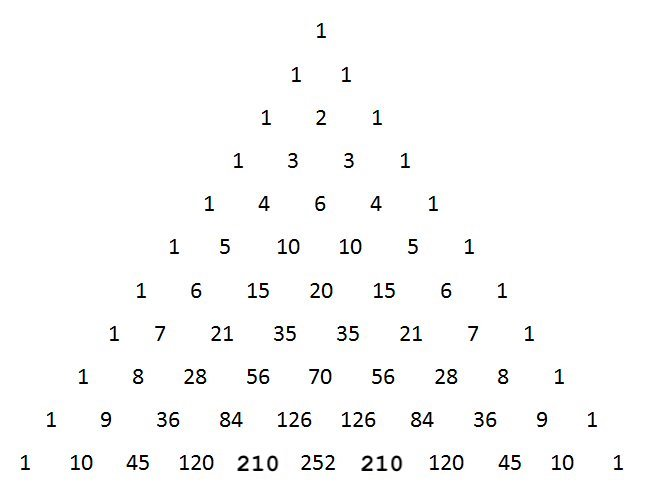
\includegraphics[width=0.75\linewidth]{Photos/Pascal's Triangle.png}
    \caption{Pascal's Triangle: A wonder of the mathematical world}    
\end{figure}
The triangle somewhere on the top of the page is called Pascal's triangle. \\
It has a lot of fun and amazing properties(try to find them, you'll be surprised).\\
We are going to exploit two of them right now. First being, Every term in subsequent line is made by adding the two above it. As it turned out, every ancient civilization did reach this triangle by doing just that. The second one, the reason Blaise Pascal gets to have his name on it.\\
\begin{figure}
    \centering
    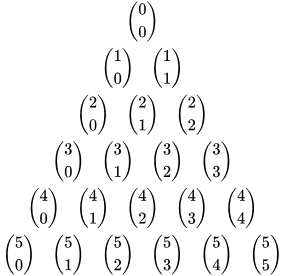
\includegraphics[width=0.75\linewidth]{Photos/Binomial Pascal}
    \caption{As it turns out, we can write everything as a binomial coefficient here.}
\end{figure}
This is exceptionally useful as this leads us to Pascal's Identity....
\begin{theorem}
    $\binom{n}{k} + \binom{n}{k+1}=\binom{n+1}{k+1}$
\end{theorem}
Remember, we saw this while proving principle of inclusion exclusion. There we proved it algebraically. We also 'proved' it in a sort of hand wavy manner above using pascal's triangle. Here is an another proof, combinatorial this time, for it.\\
\begin{proof}
    Let's consider choosing a team of $k$ lawyers from a pool of $n-1$ junior lawyers and $1$ Harvey Specter.\\
    The answer is $\binom{n}{k}$. Using casework, We can either have Harvey on the team or not on it. If Harvey is on the team, we have $\binom{n-1}{k-1}$ ways to choose rest of the lawyers. If we don't have Harvey on it, we have $\binom{n-1}{k}$ ways to choose the team.\\
    This means $\binom{n-1}{k-1}+\binom{n-1}{k}=\binom{n}{k}$.
\end{proof}
Finally, here is the hockey stick identity(try looking at a diagonal in the triangle, that's where the name comes from). We started this section at this identity, and I'll let you prove it.\\
\begin{theorem}
    $\binom{k}{k}+\binom{k+1}{k}+ \dots +\binom{n}{k}=\binom{n+1}{k+1}$
\end{theorem}
Now here is the first thing, you should remember these identities. They can be memorized quite simply by writing them on a piece of paper and taping them to a wall next to where you sleep. Every morning look at it just after you wake up, and every night just before you sleep. You'll have them memorized in less then a week.\\
The another way to remember(the one which I remember), is by simply solving the questions and deriving every identity you forget, no turning the pages back. That will get it done in less than two hours flat.\\
\section{Exercises}
Solve at least questions worth \points{60}. This exercise has a total of \points{75}.
\begin{xcb}{Exercises}
\begin{enumerate}
\item \points{2} In how many ways can one get $10$ upon rolling $7$ dice?
\item \points{2} How many $4$ digit numbers have a sum of $9$?
\item \points{3} How many ordered pairs $(a,b,c,d)$ where $a \le b \le c \le d \le 5$ and $a,b,c,d \in \mathbb{N}$?
\begin{hint}
    \addhint{Let $a=1+x$, $b=a+y$ and so on. Does this look like a Stars and Bars now?}
\end{hint}
\item (AIME 2000) \points{9} Given that\\
\[\frac 1{2!17!}+\frac 1{3!16!}+\frac 1{4!15!}+\frac 1{5!14!}+\frac 1{6!13!}+\frac 1{7!12!}+\frac 1{8!11!}+\frac 1{9!10!}=\frac N{1!18!}\]
find the greatest integer that is less than $\frac N{100}$.
\begin{hint}
    \addhint{Multiply both sides by $19!$}\\
    \addhint{Multiply both sides by $2$ and use $\binom{n}{k}=\binom{n}{n-k}$}
    \addhint{Add terms to reach an identity which we know the summation to}
\end{hint}
\item(AIME 2001) \points{3} A fair die is rolled four times. The probability that each of the final three rolls is at least as large as the roll preceding it may be expressed in the form $m/n$ where m and n are relatively prime positive integers. Find $m + n$.
\item (AMC 8 2018) \points{3} From a regular octagon, a triangle is formed by connecting three randomly chosen vertices of the octagon. What is the probability that at least one of the sides of the triangle is also a side of the octagon?
\begin{hint}
    \addhint{Can we convert the choosing of $3$ points as partitioning of remaining $5$ points into $3$?}
\end{hint}
\item(AIME 2020) \points{2} A club consisting of $11$ men and $12$ women needs to choose a committee from among its members so that the number of women on the committee is one more than the number of men on the committee. The committee could have as few as $1$ member or as many as $23$ members. Let $N$ be the number of such committees that can be formed. If $N=\binom{a}{b}$, find $a + b$
\begin{hint}
    \addhint{We'll use Vandermonde identity, now try to solve it.}
\end{hint}
\item (AIME 2015) \points{3} Consider all 1000-element subsets of the set ${{1, 2, 3, \dots , 2015}}$. From each such subset choose the least element. The arithmetic mean of all of these least elements is $p/q$, where $p$ and $q$ are relatively prime positive integers. Find $p + q$.
\begin{hint}
    \addhint{$a_1+2a_2+3a_3+\dots na_n=(a_1+a_2+\dots+a_n)+(a_2+a_3+\dots)+\dots+(a_n)$}
\end{hint}
\item \points{2} For how many positive integers $x_1, x_2, \dots, x_{10}$ do we have $x_1 + x_2 + \dots + x_{10} = 50$?
\item (AIME 2011) \points{5} Ed has five identical green marbles, and a large supply of identical red marbles. He arranges the green marbles and some of the red ones in a row and finds that the number of marbles whose right hand neighbor is the same color as themselves is equal to the number of marbles whose right hand neighbor is the other color. An example of such an arrangement is $GGRRRGGRG$. Let $m$ be the maximum number of red marbles for which such an arrangement is possible, and let $N$ be the number of ways he can arrange the $m+5$ marbles to satisfy the requirement. Find the remainder when $N$ is divided by $1000$.
\begin{hint}
    \addhint{$m$ is limited by the fact that number of marbles whose right hand neighbor is the other color is maximum 10. How many red marbles will we need for this to lead to a valid arrangement?}
    \addhint{As we know $m$ now, can we simply use stars and bars with one red marble always between 2 green.}
\end{hint}
\item (AIME 2011) \points{9} Six men and some number of women stand in a line in random order. Let $p$ be the probability that a group of at least four men stand together in the line, given that every man stands next to at least one other man. Find the least number of women in the line such that $p$ does not exceed 1 percent.
\begin{hint}
    \addhint{In what ways can the men be arranged in? Use the groups of men as bars and the women as stars}
    \addhint{Use Pascal to simplify and then open the binomial}
\end{hint}
\item \points{2} Let $n$ be a positive integer. In how many ways can one write a sum of at least two positive integers that add up to $n$?
\item (AIME 2013) \points{5} Melinda has three empty boxes and $12$ textbooks, three of which are mathematics textbooks. One box will hold any three of her textbooks, one will hold any four of her textbooks, and one will hold any five of her textbooks. If Melinda packs her textbooks into these boxes in random order, the probability that all three mathematics textbooks end up in the same box can be written as $\frac{m}{n}$, where $m$ and $n$ are relatively prime positive integers. Find $m+n$.
\begin{hint}
    \addhint{Casework onto the box in which the three math textbooks are in}
    \addhint{Simplify before you compute! Take $9!$ common, multiply numerator and denominator by $3!4!5!$}
\end{hint}
\item (AMC 10 2016) \points{3} For some particular value of $N$, when $(a + b + c + d + 1)^N$ is expanded and like terms are combined, the resulting expression contains exactly $1001$ terms that include all four variables $a, b, c,$ and $d$, each to some positive power. What is $N$?
\item (AMC 12 2021) \points{9} A choir director must select a group of singers from among his $6$ tenors and $8$ basses. The only requirements are that the difference between the number of tenors and basses must be a multiple of $4$, and the group must have at least one singer. Let $N$ be the number of different groups that could be selected. What is the remainder when $N$ is divided by $100$?
\begin{hint}
    \addhint{Casework on the tenors $-$ basses combined with Vandermonde will work.}
\end{hint}
\item (IMO 1981/2) \points{9} Let $\displaystyle 1 \le r \le n$ and consider all subsets of $\displaystyle r$ elements of the set $\{ 1, 2, \ldots , n \}$. Each of these subsets has a smallest member. Let $\displaystyle F(n,r)$ denote the arithmetic mean of these smallest numbers; prove that\\
\[F(n,r) = \frac{n+1}{r+1}.\]
\begin{hint}
    \addhint{We have already solved a case of it as an AIME 2015 problem, won't the same technique work in general?}
\end{hint}
\item \points{5} Prove that \[\sum_{k=0}^n k{\binom{n}{k}}^2=n\binom{2n-1}{n-1}\]
\end{enumerate}
\end{xcb}
\chapter{Geometrical Combinatorics}
I will not write an introduction here as my thoughts differ on both the sections.\par
While geometrical counting is a sticker to make simple questions feel difficult, geometrical probability 
is a very powerful technique which is used in research as well.\par
However, I have decided to cover them in the same chapter as they both start with the prefix 'geometric'.
\section{Geometric Counting}
\begin{example}
    [Motivating Example]
    How many rectangles of any and all sizes can be formed in a rectangular grid of size $m*n$?
\end{example}
\begin{proof}
    [Solution]
    This can simply be solved by saying that a rectangle is formed when we choose two vertical and 
    two horizontal lines.\par
    In an $m*n$ grid, we have $m+1$ verticals and $n+1$ horizontals. \par
    Hence, we can say the number of rectangles is: $\binom{m+1}{2}*\binom{n+1}{2}$
\end{proof}
This is all geometric counting is. We have a geometric 
figure and have to count something about it. It is the 
cheapest trick in the question writers tool box, if a question 
seems too simple, stick it on the top of a geometric figure and 
suddenly half the test takers will not attempt it.\par
We don't want to be those people.
\section{Geometric Probability}
Geometric probability is a way to calculate probability by measuring 
the number of outcomes geometrically, in terms of length, area, or volume. 
Why would we do that? Because sometimes, it is easier to solve for the area than 
the actual probability. We have a chocolate in India called 'Melody' which 
has a distinct chocolaty and addictive taste. Its tagline was: 
"Khud khao, khud jaan jao(Try it yourself to find it for yourself)" The same 
applies to geometric probability. Let's try it out:
\begin{example}
    [Motivating Example]
    (AMC 10 2017)Chloe chooses a real number uniformly at random from the 
    interval $[0, 2017]$. Independently, Laurent chooses a real number uniformly 
    at random from the interval $[0, 4034]$. What is the probability that Laurent’s 
    number is greater than Chloe’s number? (Assume they cannot be equal)
\end{example}
\begin{proof}
    [Solution]
    I have not provided a figure to motivate you to draw it.\par
    Let's call Chloe's number as $x$ and Laurent's number as $y$, all their choices can be 
    represented as a rectangle which is $2017$ units on the x axis and $4034$ units on the y axis. \par
    We are looking for cases where Laurent's number is greater than Chloe's, or $y>x$\par
    This is a line from $(0,0)$ to $(2017,2017)$. We can now find the area of the 
    rectangle above this line divided by the total area of the rectangle which will lead to the answer:\par
    $\frac{(2017+4034)*2017/2}{2017*4034}$\par
    $=\frac{2017*1.5}{2017*2}$\par
    $=\frac{3}{4}$
\end{proof}
Geometric probability can be useful when the number of possible outcomes is infinite and we can 
easily make a diagram to represent the outcomes.\par
Anther common type of question is:\par
\begin{example}
    A coin of radius $r$ is thrown randomly on a floor tiled with squares of side $l$. Two 
    players bet that the coin will land on exactly one or more than one square respectively. 
    What relation should $l$ and $r$ satisfy for the game to be fair? 
\end{example}
\begin{proof}
    [Solution]
    The coin lies inside the square if the center of the coin is at least $r$ distance away 
    from the boundary of the square.\par
    \begin{figure}[h]
        \centering
        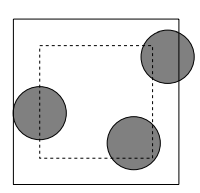
\includegraphics[width=0.5\linewidth]{Photos/Cointoss onto square.png}        
    \end{figure}
    Thus, thus the bet turns to choosing a random point inside a square. If it is at a 
    distance $d\geq r$ then player one wins or else player two wins.\par
    This means for the game to be fair:\par
    $\frac{(l-2r)^2}{l^2}=\frac{1}{2}$\par
    $\iff 2(l-2r)^2=l^2$\par
    $\iff 2l^2-8lr+8r^2=l^2$\par
    $ \iff l^2-8lr+8r^2=0$\par
    $\therefore l=\frac{8r\pm\sqrt{64r^2-32r^2}}{2}$\par
    $\iff l=\frac{8r\pm4r\sqrt{2}}{2}$\par
    $\iff l=4r\pm2r\sqrt{2}$\par
    We reject the minus case as then $l$ will be less than $r$ which is not possible.
    $\therefore l=4r+2r\sqrt{2}$
\end{proof}
In conclusion, Geometric probability is the exact converse of geometric counting.
There we used to covert a geometrical problem into a counting problem, 
here we convert a counting problem to a geometry problem. Also it was useless and unnecessary, 
while this is useful and beautiful.\par
Solve at least questions worth \points{45}. This exercise has a total of \points{60}.
\begin{xcb}{Exercises}
\begin{enumerate}
\item(AMC 10 2004) \points{2} The $5\times 5$ grid shown contains a collection of squares with sizes from $1\times 1$ to $5 \times 5$. How many of these squares contain the black center square?
\begin{center}
    \begin{tikzpicture}
  % Draw outer square
  \draw (0,0) grid (5,5);
  % Draw inner black square
  \fill[black] (2,2) rectangle (3,3);
\end{tikzpicture}
\end{center}
\begin{hint}
    \addhint{Just count!}
\end{hint}
\item(Extension to 1) \points{3} How many rectangles formed by the grid lines in this $5\times 5$ grid contain the black center square?
\item(AMC 10 2007) \points{3} A set of $25$ square blocks is arranged into a $5*5$ square. How many different combinations of $3$ blocks can be selected from that set so that no two are in the same row or column?
\item(AMC 10 2021) \points{3} How many ways are there to place $3$ indistinguishable red chips, $3$ indistinguishable blue chips, and $3$ indistinguishable green chips in the squares of a $3$ by $3$ grid so that no two chips of the same color are directly adjacent to each other, either vertically or horizontally?
\begin{hint}
    \addhint{The cases seem to be less enough that maybe just counting for one colour followed by some multiplication is good sauce.}
\end{hint}
\item (AIME 2006) \points{5} There is an unlimited supply of congruent equilateral triangles made of colored paper. Each triangle is a solid color with the same color on both sides of the paper. A large equilateral triangle is constructed from four of these paper triangles. Two large triangles are considered distinguishable if it is not possible to place one on the other, using translations, rotations, and/or reflections, so that their corresponding small triangles are of the same color. Given that there are six different colors of triangles from which to choose, how many distinguishable large equilateral triangles may be formed?
\begin{hint}
    \addhint{Focus on the color of the center triangle}
    \addhint{Case work onto number of same color triangles on the outside.}
\end{hint}
\item (AMC 10 2019) \points{5} Real numbers between $0$ and $1$, inclusive, are chosen in the following manner. A fair coin is flipped. If it lands heads, then it is flipped again and the chosen number is $0$ if the second flip is heads, and 1 if the second flip is tails. On the other hand, if the first coin flip is tails, then the number is chosen uniformly at random from the closed interval $[0, 1]$. Two random numbers x and y are chosen independently in this manner. What is
the probability that $|x - y| > \frac{1}{2}$?
\begin{hint}
    \addhint{Case work onto the possible coin flips results}
\end{hint}
\item (AIME 2004) \points{3} A circle of radius $1$ is randomly placed in a $15 \times 36$ rectangle ABCD so that the circle lies completely within the rectangle. Given that the probability that the circle will not touch diagonal AC is $m/n$, where m and n are relatively prime positive integers. Find $m + n$.
\item (AIME 1989) \points{2} $10$ points are marked on a circle. How many distinct convex polygons can be made using a subset of them as vertices?
\item \points{3} There are $10$ points on the circumference of a circle. How many points of intersection of line segments with ends at these points will be inside the circle?
\begin{hint}
    \addhint{While some lines will intersect outside, won't every four points give us a pair of two lines intersecting inside?}
\end{hint}
\item \points{2} There are 6 points on the x axis and 9 points on the y axis. How many points of intersection of these points lie in  the first quadrant?
\item \points{2} There are 10 lines in a plane, with no three being concurrent and no two being parallel. How many triangles can be formed using there points of intersection?
\item \points{2} Sheldon is standing at (0,0,0) and can move one unit along either the x, y or z axis. IN how many ways can he walk up to (3,3,3)?
\item \points{9} Choose $n$ points randomly from a circle, What is the probability that all the points are in one semicircle?
\begin{hint}
    \addhint{Choose one point as reference which is one of the diameter points of the semi-circle, we can lie on either side of the diameter.}
    \addhint{We have $n$ possible reference points}
\end{hint}
\item (Amazon Interview) \points{9} A stick is broken in two random places. What are the odds that the three pieces can form the sides of a triangle? 
\begin{hint}
    \addhint{Take the sides as $x,y-x,n-y$ where $n$ is the length of the stick.}
\end{hint}
\item (OMCC 2003) \points{9} A square board with side-length of $8$ cm is divided into $64$ squares with side-length of $1$ cm each. Each square can be painted black or white. Find the total number of ways to color the board so that every square with side-length of $2$ cm formed with $4$ small squares with a common vertex has two black squares and two white squares.
\begin{hint}
    \addhint{Try fixing a column}
    \addhint{If we get a BB or WW in a column, the other is determined uniquely}
\end{hint}
\end{enumerate}
\end{xcb}
\backmatter
\part{Appendix}
%% References
\clearpage
\end{document}
